% Created 2022-01-09 Sun 10:20
% Intended LaTeX compiler: pdflatex
\documentclass[bigger]{beamer}
\usepackage[utf8]{inputenc}
\usepackage[T1]{fontenc}
\usepackage{graphicx}
\usepackage{grffile}
\usepackage{longtable}
\usepackage{wrapfig}
\usepackage{rotating}
\usepackage[normalem]{ulem}
\usepackage{amsmath}
\usepackage{textcomp}
\usepackage{amssymb}
\usepackage{capt-of}
\usepackage{hyperref}
\mode<beamer>{\usetheme{Madrid}}
\usetheme{default}
\author{Eric S Fraga}
\date{2010-03-30 Tue}
\title{Writing Beamer presentations in org-mode}
\hypersetup{
 pdfauthor={Eric S Fraga},
 pdftitle={Writing Beamer presentations in org-mode},
 pdfkeywords={},
 pdfsubject={},
 pdfcreator={Emacs 27.2 (Org mode 9.4.4)}, 
 pdflang={English}}
\begin{document}

\maketitle
\begin{frame}{Outline}
\tableofcontents
\end{frame}



\section{Introduction}
\label{sec:org5c56c10}
\begin{frame}[label={sec:orgdc24886},fragile]{Preface}
 This is an updated file based on \href{https://orgmode.org/worg/exporters/beamer/tutorial.html}{this tutorial} from Eric S Fraga in an attempt to clarify
org-mode Beamer export in 2022 for \href{https://stackoverflow.com/questions/6691588/emacs-org-beamer-no-definition-for-class-beamer-in-org-export-latex-class/7972859}{this StackExchange question}.

Key changes:
\begin{itemize}
\item had to change \texttt{H:3} to \texttt{H:2} in the \texttt{\#+options} line
\item added in the Madrid template
\item deleted options lines that didn't seem relevant
\item regenerated a screenshot so the image insertion would work
\item made a \texttt{min-config} for reproducibility; one should \texttt{emacs -Q}, then \texttt{M-x load-file
  [RET] path/to/min-config} and then try exporting
\end{itemize}
\end{frame}

\begin{frame}[label={sec:org9d87f98},fragile]{Overview}
 This presentation provides an illustration of some of the capabilities of the \alert{Beamer} export in \texttt{org} mode:

\begin{enumerate}
\item simple slides (this one),
\item slides with special blocks,
\item multi-column slides and
\item the use of \alert{Babel} for literate programming.
\end{enumerate}

This file should be exported using \texttt{M-x org-export-dispatch} (\texttt{C-c C-e}), specifying \texttt{l} for \LaTeX{} and then \texttt{P}, for instance, to generate the PDF.
\end{frame}

\section{Methodology}
\label{sec:orgab466d8}
\begin{frame}[label={sec:org62a74ca},fragile]{A simple slide}
 This slide consists of some text with a number of bullet points:

\begin{itemize}
\item the first, very \alert{important}, point!
\item the previous point shows the use of the special markup which
translates to the Beamer specific \emph{alert} command for highlighting
text.
\item note: the original worg presentation features \texttt{@foo@} notation for the very
\texttt{@important@} point above, which is supposed to convert the text to \texttt{\textbackslash{}alert\{foo\}}, but
isn't happening. I can't find information easily on why and just replaced it with bold text.
\end{itemize}

The above list could be numbered or any other type of list and may
include sub-lists.
\end{frame}

\begin{frame}[label={sec:org1eeda91}]{A more complex slide}
This slide illustrates the use of Beamer blocks.  The following text,
with its own headline, is displayed in a block:

\begin{theorem}[Org mode increases productivity]
\begin{itemize}
\item org mode means not having to remember \LaTeX{} commands.
\item it is based on ascii text which is inherently portable.
\item Emacs!
\end{itemize}

\hfill \(\qed\)
\end{theorem}
\end{frame}


\begin{frame}[label={sec:org4210a3e}]{Two columns}
\begin{columns}
\begin{column}{0.4\columnwidth}
\begin{itemize}
\item this slide consists of two columns
\item the first (left) column has no heading and consists of text
\item the second (right) column has an image and is enclosed in an
\alert{example} block
\end{itemize}
\end{column}

\begin{column}{0.6\columnwidth}
\begin{example}[A screenshot]
\begin{center}
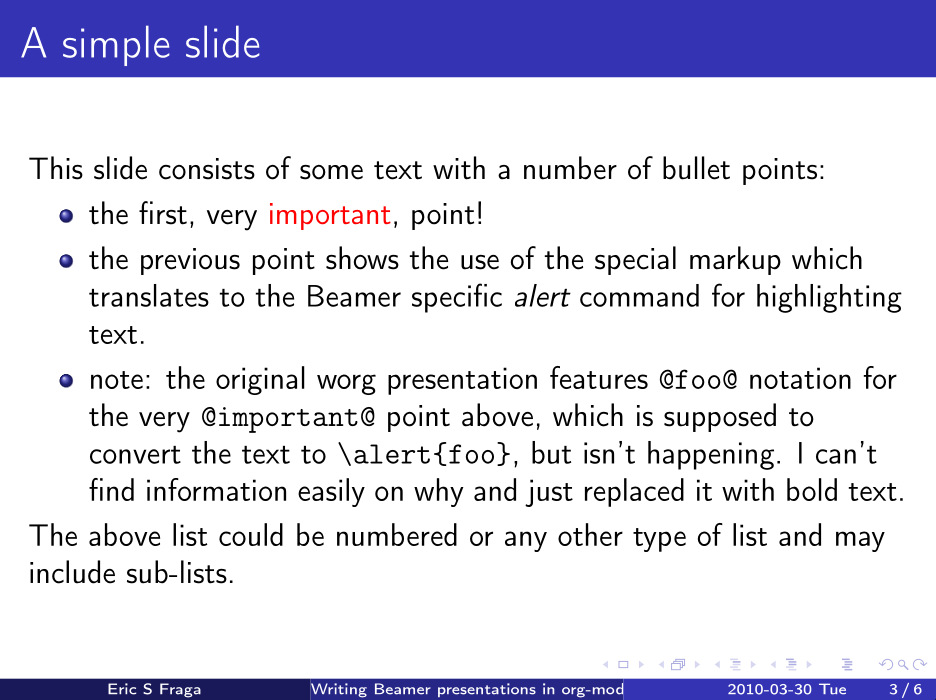
\includegraphics[width=.9\linewidth]{./img/a_simple_slide.png}
\end{center}
\end{example}
\end{column}
\end{columns}
\end{frame}


\begin{frame}[label={sec:orgf9f5b82},fragile]{Babel}
 \begin{columns}
\begin{column}{0.45\columnwidth}
\begin{block}{Octave code}
\begin{verbatim}
A = [1 2 ; 3 4]
b = [1; 1];
x = A\b
\end{verbatim}
\end{block}
\end{column}

\begin{column}{0.4\columnwidth}
\begin{block}{The output}
\begin{verbatim}
A =

   1   2
   3   4

x =

  -1
   1

\end{verbatim}
\end{block}
\end{column}
\end{columns}
\end{frame}

\section{Conclusions}
\label{sec:org24b7f15}

\begin{frame}[label={sec:orgb364d32}]{Summary}
\begin{itemize}
\item org is an incredible tool for time management
\item \alert{but} it is also excellent for writing and for preparing presentations
\item Beamer is a very powerful \LaTeX{} package for presentations
\item the combination is unbeatable!
\end{itemize}
\end{frame}
\end{document}
